\section{Desarrollo de la solución}

\subsection{Avance en Backend}

\subsection{Avance en End-point}

\subsection{Avance en Frontend}

En esta segunda etapa de implementación se ha llevado a cabo el
desarrollo de la interfaz de usuario, la cual fue desarrollada en
Ruby on Rails bajo un patrón de arquitectura modelo-vista-controlador
(MVC).

Actualmente el sitio que aloja el Observatorio Virtual es
\url{http://beta.chivo.cl/} (como lo muestra la Fig.~\ref{img:chivo}),
el cual está compuesto por una página principal que contiene las
últimas noticias relacionadas al mundo de la astronomía y la
informática, junto con un resumen de las instituciones participantes y
una breve descripción del proyecto. Además cuenta con secciones donde
se detalla a todos los participantes del proyecto a nivel
institucional y personal, las noticias y descripciones del proyecto y
definiciones de un observatorio virtual, entre otros.

\begin{figure}[ht!]
    \begin{center}
	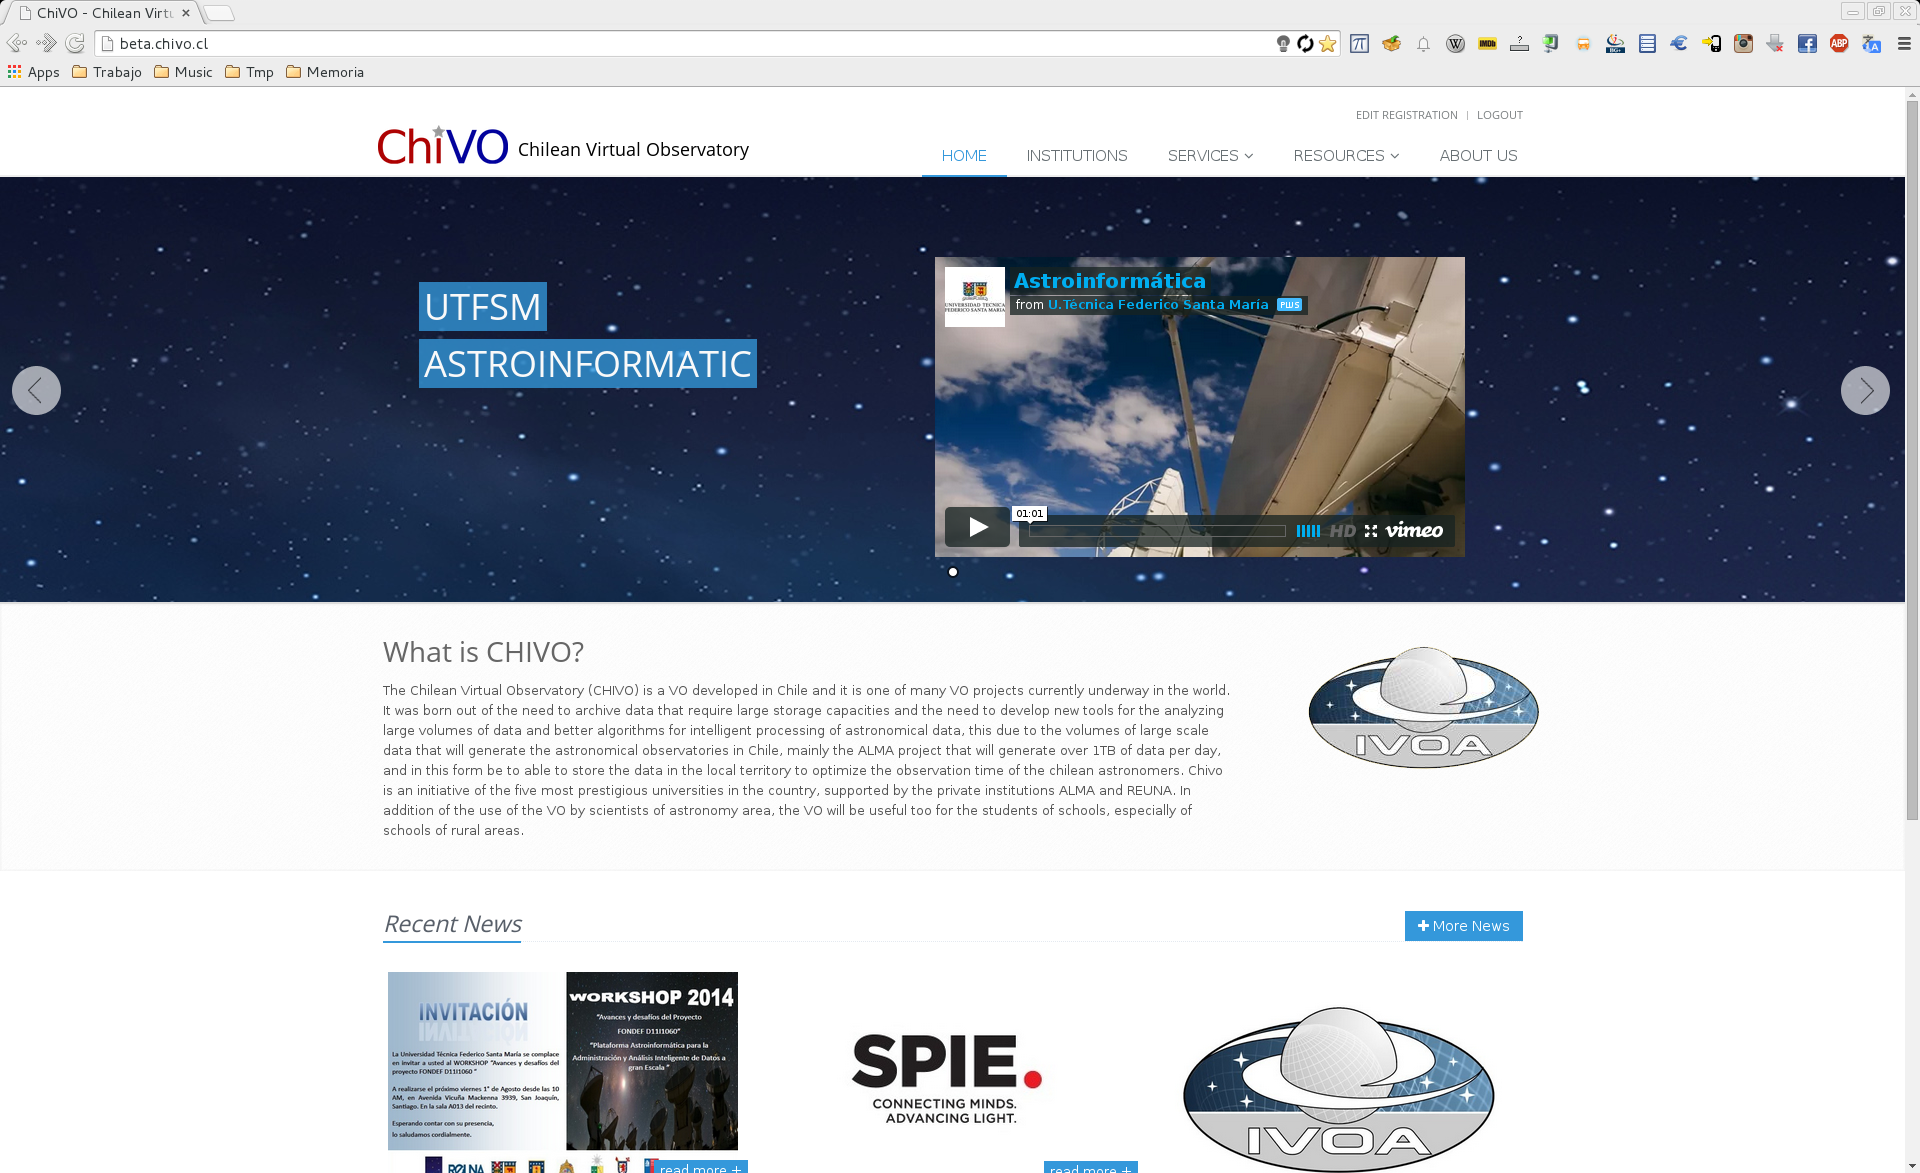
\includegraphics[scale=.2]{img/chivo}
    \end{center}
    \caption{Sitio del \emph{Chilean Virtual Observatory} en su
      versión beta.}\label{img:chivo}
\end{figure}

Por otro lado, se encuentra una sección (\emph{services}) dedicada a
realizar diferentes tipos de búsquedas según los protocolos
recomendados por IVOA\footnote{International Virtual Observatory
Alliance: \url{http://www.ivoa.net/}.}. Aquí se encontrará
específicamente 3 búsquedas: \emph{Simple Cone Search}, \emph{Simple
Image Access} y \emph{Simple Spectral Access}, además de un tipo de
búsqueda denominada \emph{all search}, que busca cumplir con los
requerimientos del mandante de este proyecto (ALMA), y que tiene por
objetivo emular el servicio \emph{ALMA Science Archive
Query}\footnote{\url{https://almascience.nrao.edu/aq/}.}. Esta última
sección no se encuentra dentro del marco de esta segunda
implementación, pues está basada bajo los estándares IVOA. No
obstante, se puede observar algunos tipos de búsquedas que ya han sido
implementadas.

A continuación se describe el desarrollo de cada una de las búsquedas
actualmente soportadas por ChiVO.


\subsubsection{Simple Cone Search}

Para acceder a esta búsqueda, se debe ingresar al menú superior
\emph{services} y seleccionar la opción \emph{cone search}, o ir
directamente a la dirección
\url{http://beta.chivo.cl/query/conesearch}. Allí se desplegará un
formulario con los datos requeridos para realizar la búsqueda, como se
muestra en la Fig.\ref{img:scs}.

\begin{figure}[ht!]
    \begin{center}
	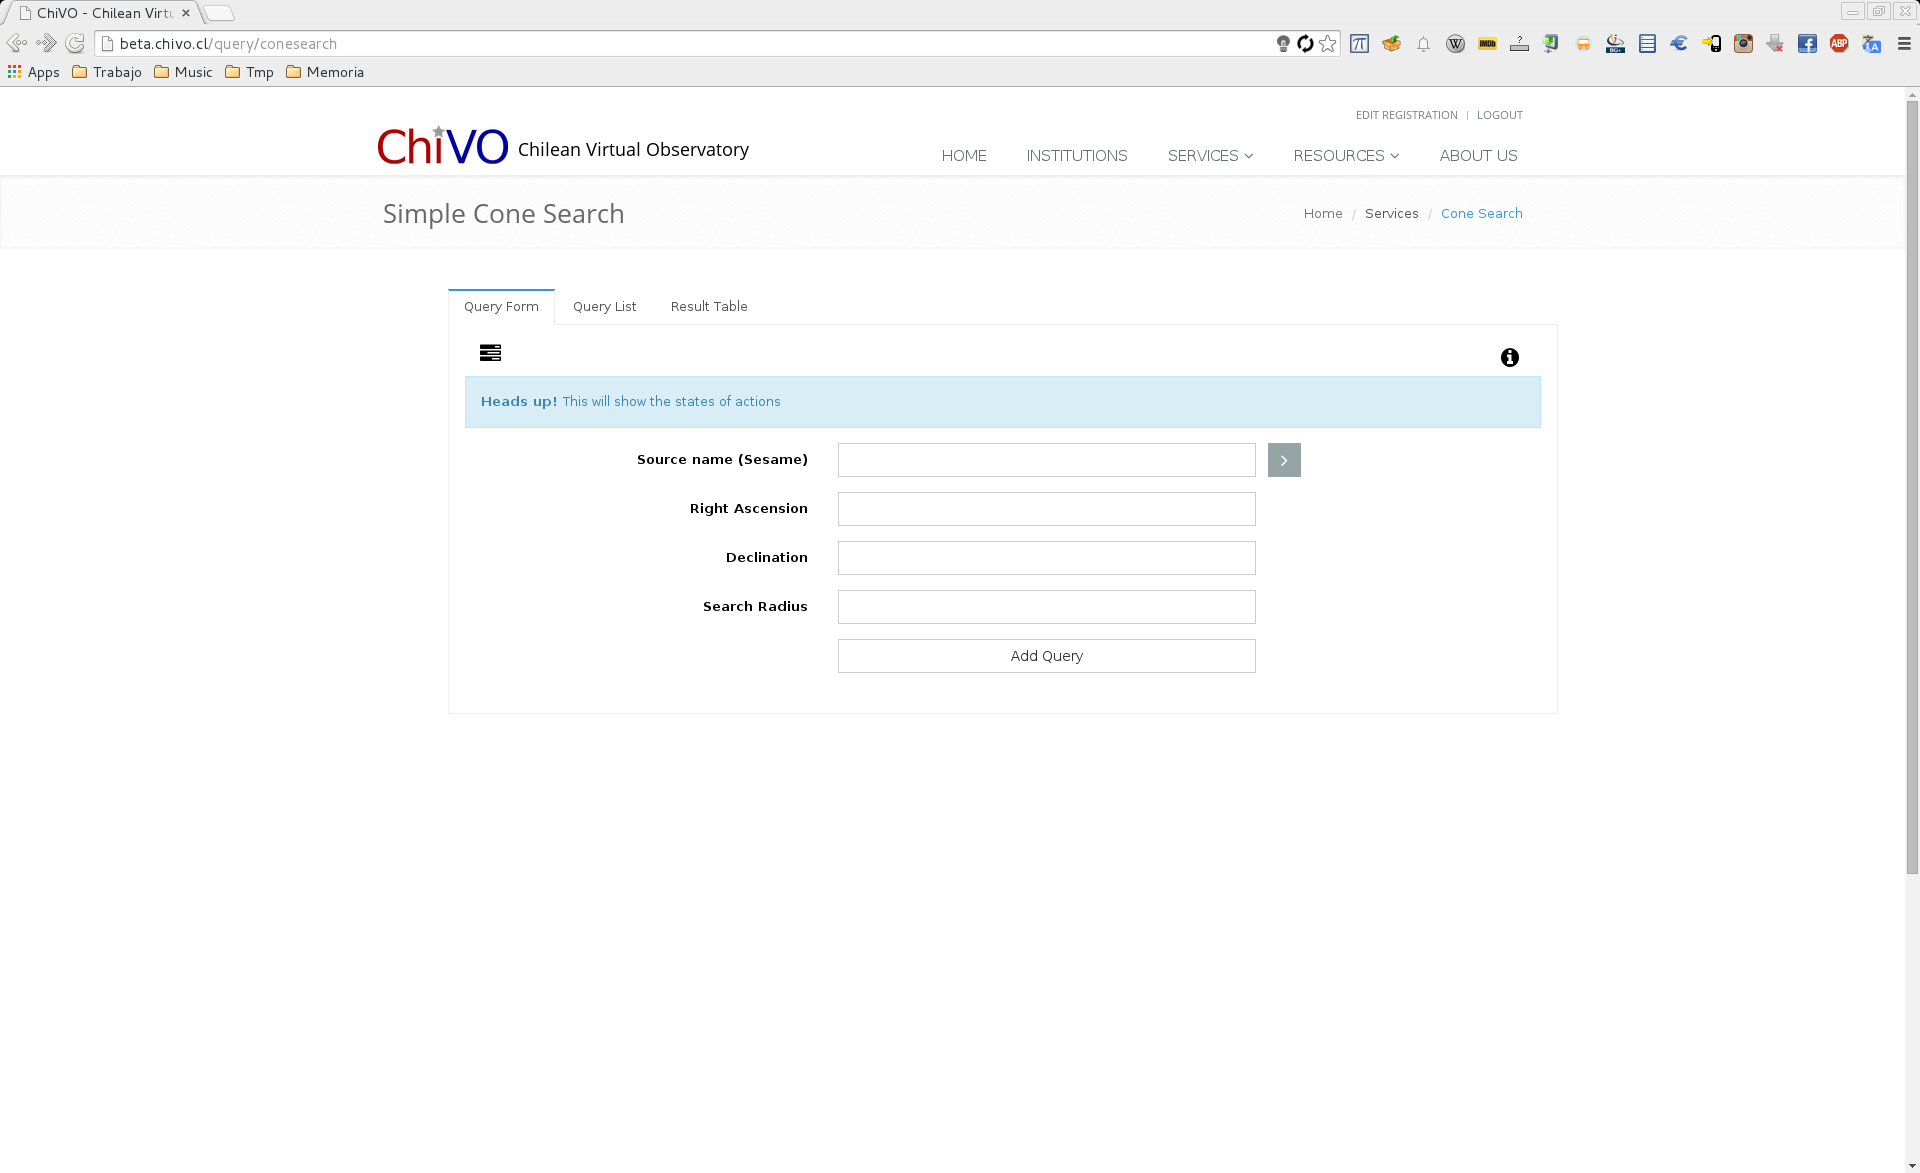
\includegraphics[scale=.2]{img/scs}
    \end{center}
    \caption{\emph{Simple Cone Search}.}\label{img:scs}
\end{figure}

Esta vista, tiene la característica de estar separada en 3 pestañas:
\emph{Query Form} (formulario de consulta), \emph{Query List} (lista
de consultas) y \emph{Result Table} (tabla de resultados). En las dos
primeras se podrá encontrar un ícono con la letra ``i'', el cual tiene
por objetivo mostrar una breve descripción que ayude al usuario a
entender qué significa cada campo. Si se presiona este ícono, los
campos en el formulario tomarán otro color, y con sólo posicionar el
cursor del ratón sobre uno de ellos se desplegará la ayuda. Además,
justo bajo el ícono de información se deplegará un mensaje por cada
acción ejecutada. En un comienzo, el primer mensaje resaltado será
\emph{Heads up! This will show the states of actions} (¡Ayuda! Esto
mostrará los estados de las acciones), avisando que allí se mostrará
una pequeña reseña por cada acción ejecutada.

A continuación se describirá el funcionamiento desarrollado para cada
una de las pestañas en esta búsqueda.

\begin{description}
  \item [Query Form:] este formulario de consulta permite ingresar los
    datos necesarios para poder realizar la búsqueda. Una vez
    ingresado los datos en los campos correspondientes, se debe
    presionar el botón \emph{Add Query} (agregar consulta) para
    agregar la consulta a la lista de consultas. Una vez hecho esto,
    se debe pasar a la siguiente pestaña, \emph{Query List}. Los
    campos presentes en este formulario son:
    \begin{description}
      \item [Source name (Sesame):] corresponde a un resolvedor de
	nombres. Los objetos astronómicos poseen en su mayoría un
	nombre común de fácil aprendizaje, el cual puede ser ingresado
	en este campo y automáticamente el sistema completará los
	datos de RA \& DEC. Actualmente se utiliza el Sesame de
	{\ldots}, pero se trabaja en la construcción de uno propio.
      \item [Right Ascension:] es la distancia angular medida hacia el
	este a lo largo del ecuador celeste desde el equinoccio de
	primavera al círculo horario del punto en cuestión. La unidad
	de medida permita es horas:minutos:segundos y grados:minutos:segundos.
      \item [Declination:] es uno de los dos ángulos que localizan un
	punto de la esfera celeste en el sistema de coordenadas
	ecuatorial. La unidad de medida permitida es
	grados:arcominutos:arcosegundos.
      \item [Search Radius:] corresponde al radio de búsqueda dentro
	del área delimitada por RA \& DEC.
    \end{description}
  \item [Query List:] una vez ingresada la consulta en la pestaña
    anterior (\emph{Query Form}), luego de presionar el botón
    \emph{Add Query}, en esta pestaña aparecerá un listado con las
    consultas ingresadas y listas para ser procesadas. En esa lista
    aparecerá los campos ingresados en la pestaña anterior, además de
    un listado con las fuentes de información.
    \begin{description}
      \item [Sources:] corresponde al listado con las fuentes de
	información que contienen los datos solicitados. Acá debe ser
	seleccionada a lo menos una para ser procesada y así el
	sistema pueda entregar una respuesta.
    \end{description}
  \item [Result Table:] luego de presionar el botón \emph{process} en
    la pestaña anterior (\emph{Query List}), en esta pesataña
    aparecerá un listado con las fuentes consultadas. Cada una de las
    fuentes corresponderá a un botón el cual puede ser presionado para
    desplegar los resultados correspondientes en el formato
    recomendado por IVOA, \emph{VOTable}.
\end{description}  


\subsubsection{Simple Image Access}

Para acceder a esta búsqueda, se debe ingresar al menú superior
\emph{services} y seleccionar la opción \emph{Image Search}, o ir
directamente a la dirección
\url{http://beta.chivo.cl/query/imagesearch}. Allí se desplegará un
formulario con los datos requeridos para realizar la búsqueda, como se
muestra en la Fig.~\ref{img:sia}

\begin{figure}[ht!]
    \begin{center}
	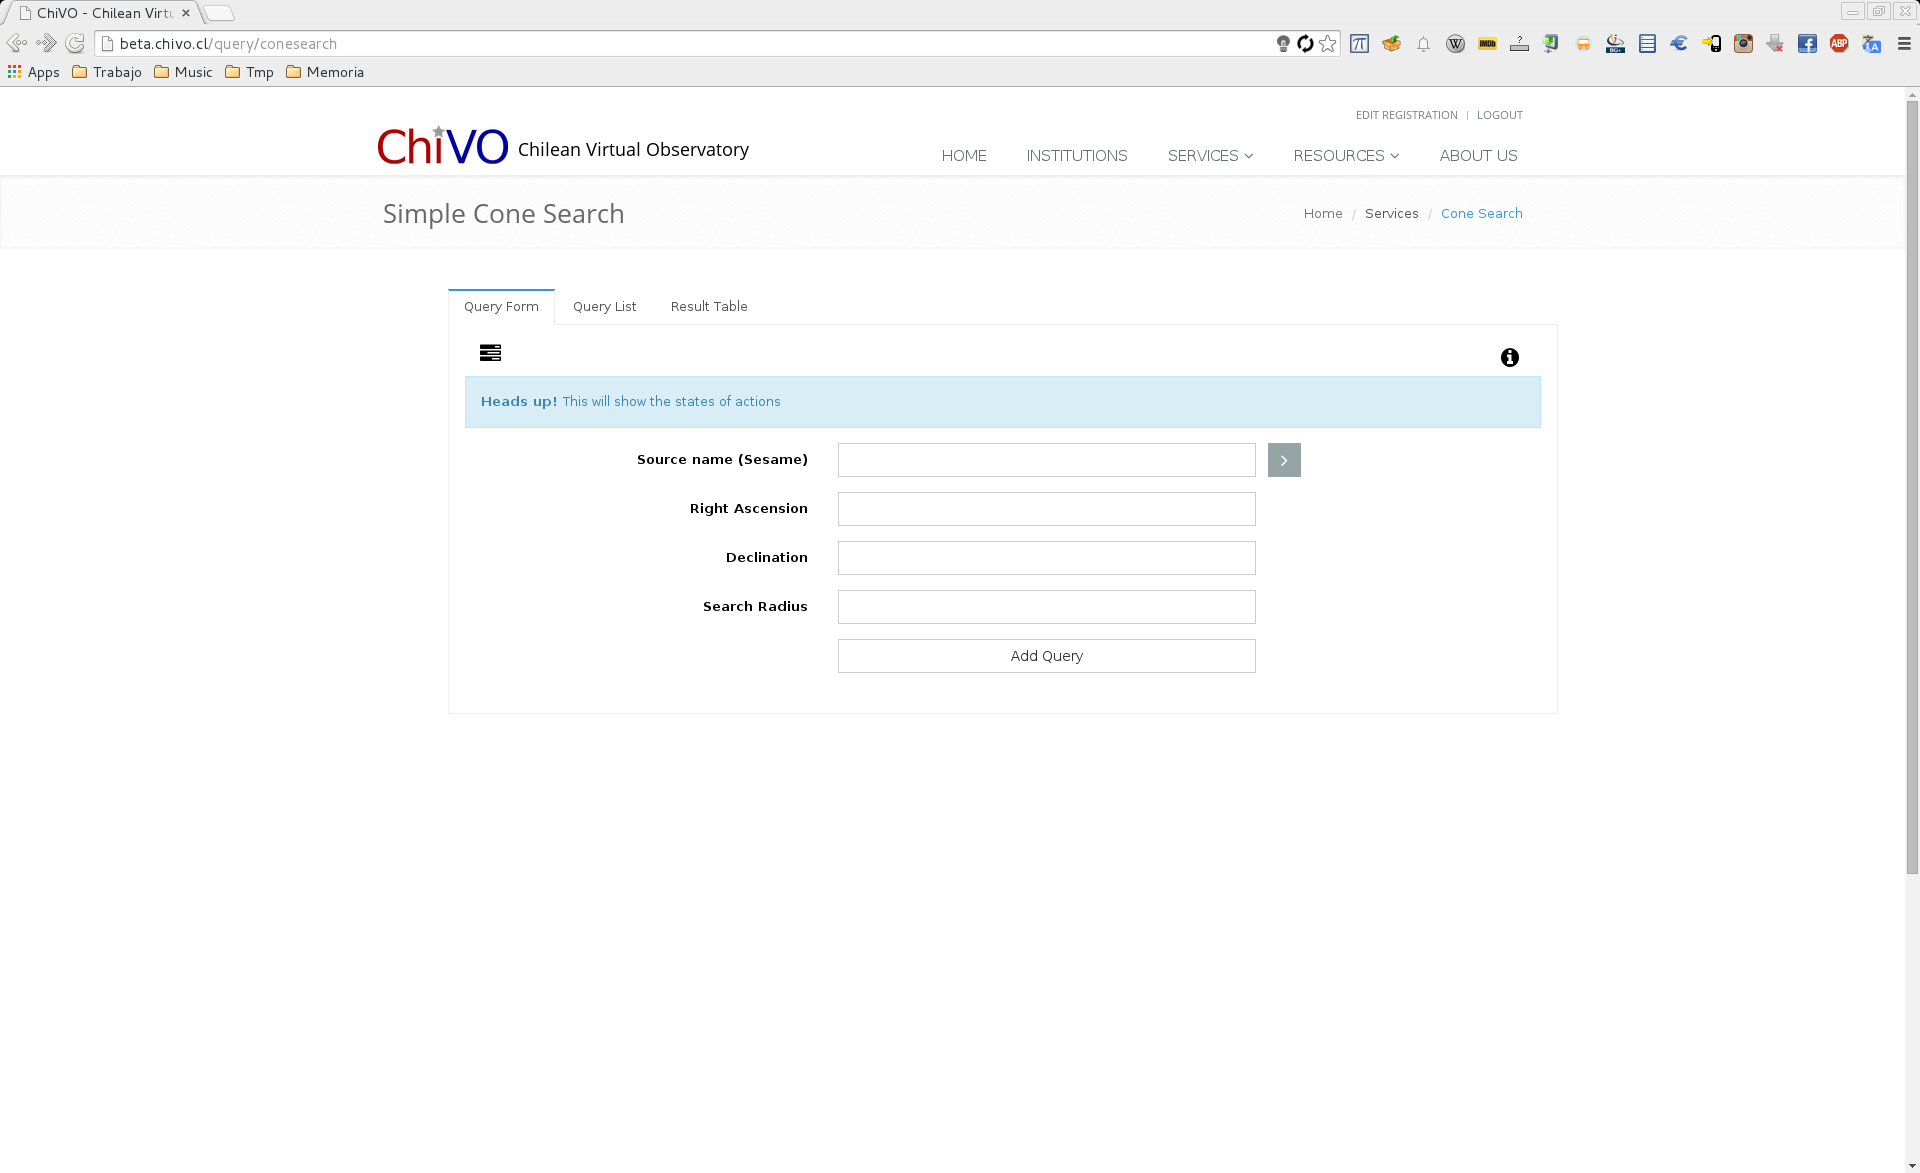
\includegraphics[scale=.2]{img/sia}
    \end{center}
    \caption{\emph{Simple Image Access}.}\label{img:sia}
\end{figure}

Al igual que la búsqueda anterior, para el protocolo \emph{Simple
Image Access} existe una vista con 3 pestañas, con exactamente la
misma estructura: \emph{Query Form}, \emph{Query List} y \emph{Query
Results}. En las dos primeras existe un ícono con la letra ``i'', que
al presionarlo, se pasa al modo de ayuda en el formulario, cuyos
campos cambian de color y despliegan información con sólo posicionar
el cursor del ratón sobre cada uno. También existe una barra con
mensajes de ayuda respecto a cada acción ejecutada. Al ingresar a esta
búsqueda, el primer mensaje que se observará será el siguiente:
\emph{Heads up! This will show the states of actions} (¡Ayuda! Esto
mostrará el estado de las acciones). Luego de ejecutar alguna acción,
en el mismo lugar de este mensaje se deplegará otra información de
interés.

A continuación se describirá el funcionamiento desarrollado para cada
una de las pestañas en esta búsqueda.

\begin{description}
  \item [Query Form:] este formulario de consulta permite ingresar los
    datos necesarios para poder realizar la búsqueda. Una vez
    ingresado los datos en los campos correspondientes, se debe
    presionar el botón \emph{Add Query} (agregar consulta) para
    agregar la consulta a la lista de consultas. Una vez hecho esto,
    se debe pasar a la siguiente pestaña, \emph{Query List}. Los
    campos presentes en este formulario son:
    \begin{description}
      \item [Source name (Sesame):] corresponde a un resolvedor de
	nombres. Los objetos astronómicos poseen en su mayoría un
	nombre común de fácil aprendizaje, el cual puede ser ingresado
	en este campo y automáticamente el sistema completará los
	datos de RA \& DEC. Actualmente se utiliza el Sesame de
	{\ldots}, pero se trabaja en la construcción de uno propio.
      \item [RA:] \emph{Right Ascension} es la distancia angular
	medida hacia el este a lo largo del ecuador celeste desde el
	equinoccio de primavera al círculo horario del punto en
	cuestión. La unidad de medida permita es
	horas:minutos:segundos y grados:minutos:segundos.
      \item [DEC:] \emph{Declination} es uno de los dos ángulos que
	localizan un punto de la esfera celeste en el sistema de
	coordenadas ecuatorial. La unidad de medida permitida es
	grados:arcominutos:arcosegundos.
      \item [Angular Size:] 
      \item [Optional parameters:] los parámetros opcionales
	corresponden a una lista de parámetros que no son necesarios
	para realizar la búsqueda. Sólo sirven si se requiere afinar
	con más detalles la búsqueda.
      \item [Intersect:]
      \item [N Axis:]
      \item [C Frame:]
      \item [Rotang:]
      \item [Proj:]
      \item [Data Type:]
      \item [Verbosity:]
      \item [Import CSV File:]
    \end{description}  
  \item [Query List:] una vez ingresada la consulta en la pestaña
    anterior (\emph{Query Form}), luego de presionar el botón
    \emph{Add Query}, en esta pestaña aparecerá un listado con las
    consultas ingresadas y listas para ser procesadas. En esa lista
    aparecerá los campos ingresados en la pestaña anterior, además de
    un listado con las fuentes de información.
    \begin{description}
      \item [Sources:] corresponde al listado con las fuentes de
	información que contienen los datos solicitados. Acá debe ser
	seleccionada a lo menos una para ser procesada y así el
	sistema pueda entregar una respuesta.
    \end{description}  
  \item [Query Results:] luego de presionar el botón \emph{process} en
    la pestaña anterior (\emph{Query List}), en esta pestaña
    aparecerá un listado con las fuentes consultadas. Cada una de las
    fuentes corresponderá a un botón el cual puede ser presionado para
    desplegar los resultados correspondientes en el formato
    recomendado por IVOA, \emph{VOTable}.
\end{description}


\subsubsection{Simple Spectral Access}

Para acceder a esta búsqueda, se debe ingresar al menú superior
\emph{services} y seleccionar la opción \emph{Spectral Search}, o ir
directamente a la dirección
\url{http://beta.chivo.cl/query/spectralsearch}. Allí se desplegará un
formulario con los datos requeridos para realizar la búsqueda, como se
muestra en la Fig.~\ref{img:ssa}

\begin{figure}[ht!]
    \begin{center}
	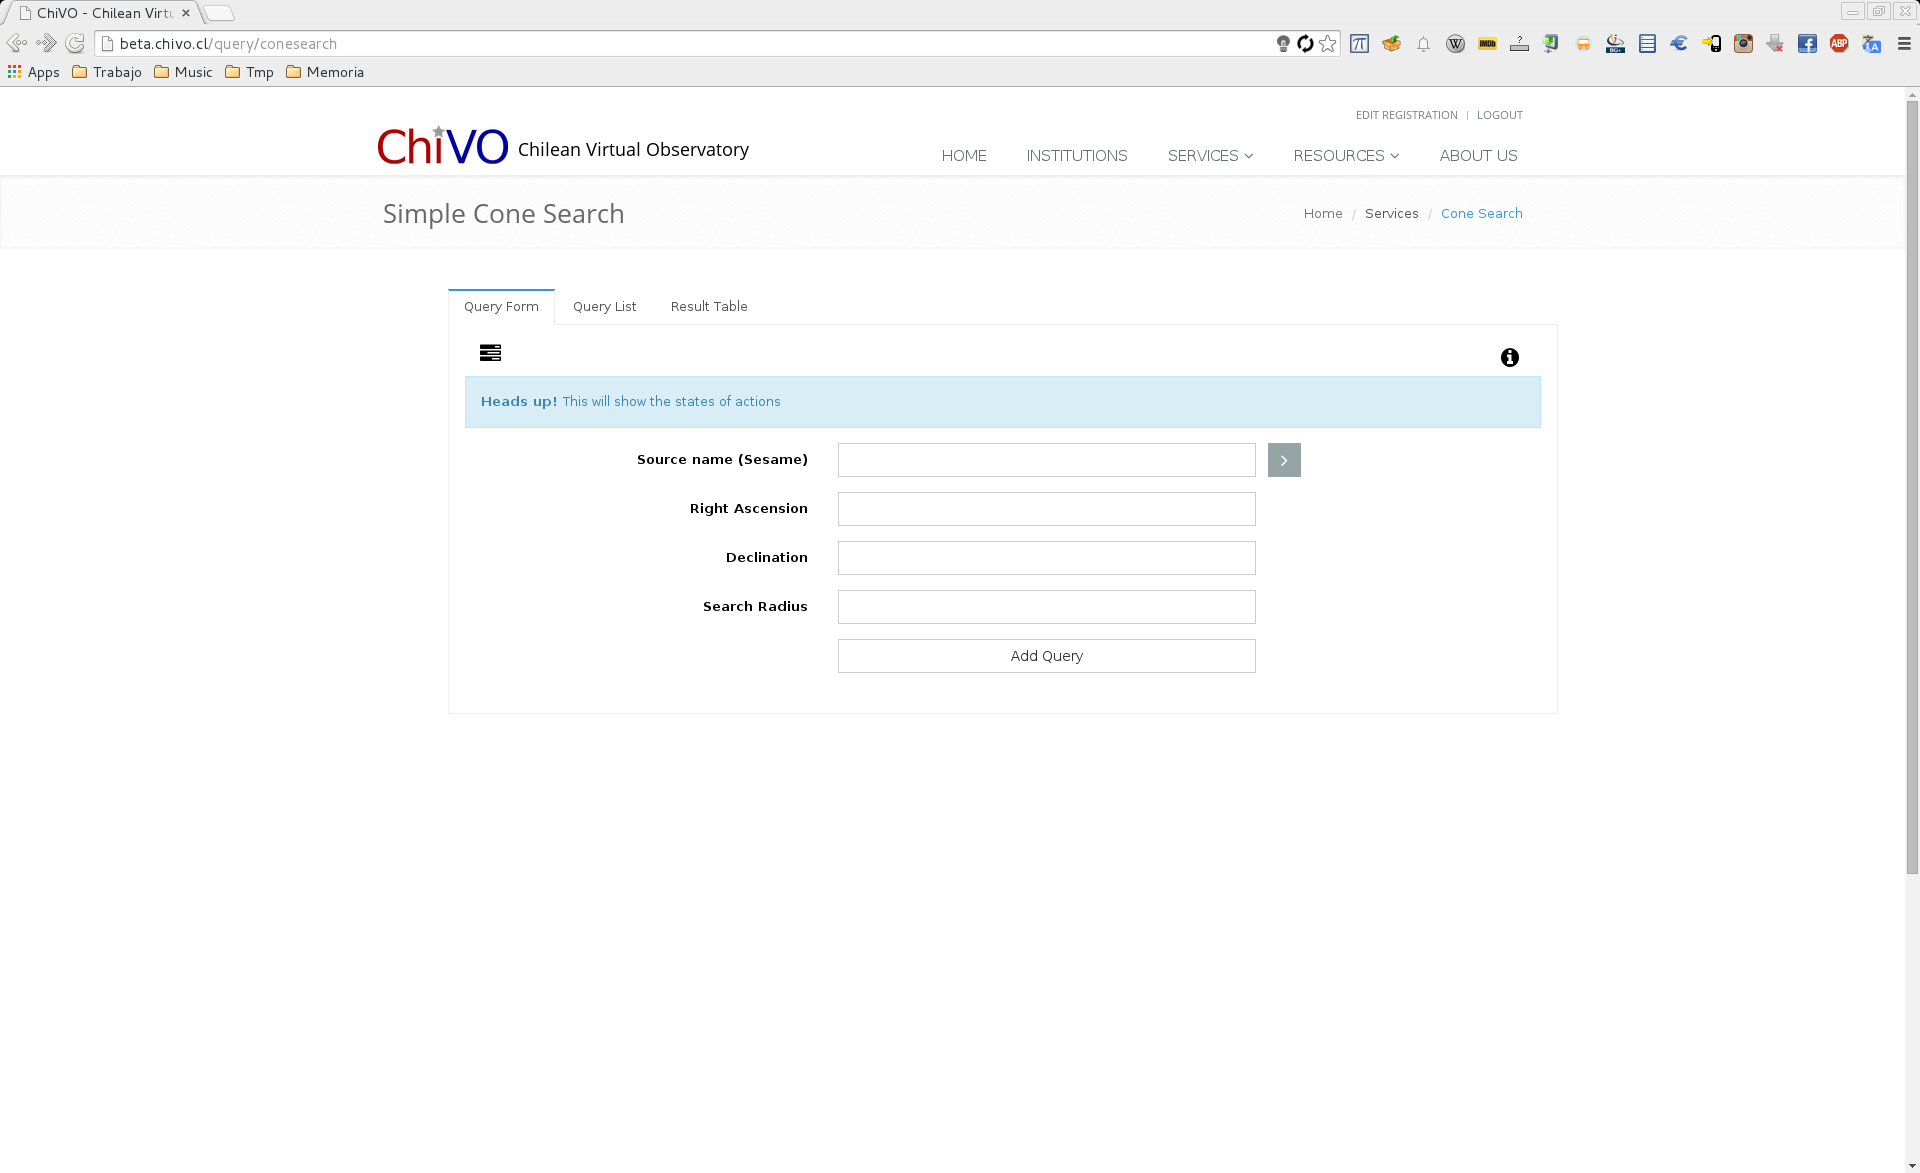
\includegraphics[scale=.2]{img/ssa}
    \end{center}
    \caption{\emph{Simple Spectral Access}.}\label{img:ssa}
\end{figure}

Al igual que en las búsquedas anteriores, para el protocolo \emph{Simple
Spectral Access} existe una vista con 3 pestañas, con exactamente la
misma estructura: \emph{Query Form}, \emph{Query List} y \emph{Query
Results}. En las dos primeras existe un ícono con la letra ``i'', que
al presionarlo, se pasa al modo de ayuda en el formulario, cuyos
campos cambian de color y despliegan información con sólo posicionar
el cursor del ratón sobre cada uno. También existe una barra con
mensajes de ayuda respecto a cada acción ejecutada. Al ingresar a esta
búsqueda, el primer mensaje que se observará será el siguiente:
\emph{Heads up! This will show the states of actions} (¡Ayuda! Esto
mostrará el estado de las acciones). Luego de ejecutar alguna acción,
en el mismo lugar de este mensaje se deplegará otra información de
interés.

A continuación se describirá el funcionamiento desarrollado para cada
una de las pestañas en esta búsqueda.

\begin{description}
  \item [Query Form:] este formulario de consulta permite ingresar los
    datos necesarios para poder realizar la búsqueda. Una vez
    ingresado los datos en los campos correspondientes, se debe
    presionar el botón \emph{Add Query} (agregar consulta) para
    agregar la consulta a la lista de consultas. Una vez hecho esto,
    se debe pasar a la siguiente pestaña, \emph{Query List}. Los
    campos presentes en este formulario son:
    \begin{description}
      \item [Source name (Sesame):] corresponde a un resolvedor de
	nombres. Los objetos astronómicos poseen en su mayoría un
	nombre común de fácil aprendizaje, el cual puede ser ingresado
	en este campo y automáticamente el sistema completará los
	datos de RA \& DEC. Actualmente se utiliza el Sesame de
	{\ldots}, pero se trabaja en la construcción de uno propio.
      \item [Right Ascension:] ascensión recta es la distancia angular
	medida hacia el este a lo largo del ecuador celeste desde el
	equinoccio de primavera al círculo horario del punto en
	cuestión. La unidad de medida permita es
	horas:minutos:segundos y grados:minutos:segundos.
      \item [Declination:] declinación es uno de los dos ángulos que
	localizan un punto de la esfera celeste en el sistema de
	coordenadas ecuatorial. La unidad de medida permitida es
	grados:arcominutos:arcosegundos.
      \item [Size:] 
      \item [Band:]
      \item [Time:]
    \end{description}  
  \item [Query List:] una vez ingresada la consulta en la pestaña
    anterior (\emph{Query Form}), luego de presionar el botón
    \emph{Add Query}, en esta pestaña aparecerá un listado con las
    consultas ingresadas y listas para ser procesadas. En esa lista
    aparecerá los campos ingresados en la pestaña anterior, además de
    un listado con las fuentes de información.
    \begin{description}
      \item [Sources:] corresponde al listado con las fuentes de
	información que contienen los datos solicitados. Acá debe ser
	seleccionada a lo menos una para ser procesada y así el
	sistema pueda entregar una respuesta.
    \end{description}  
  \item [Query Results:] luego de presionar el botón \emph{process} en
    la pestaña anterior (\emph{Query List}), en esta pestaña
    aparecerá un listado con las fuentes consultadas. Cada una de las
    fuentes corresponderá a un botón el cual puede ser presionado para
    desplegar los resultados correspondientes en el formato
    recomendado por IVOA, \emph{VOTable}.
\end{description}


\subsection{Integración}

Luego del desarrollo realizado por los 3 equipos de \emph{backend},
\emph{endpoint} y \emph{frontend}, se ha llevado a cabo un trabajo
mancomunado que ha dado como resultado la implementación de las 3
búsquedas presentes actualmente en el sistema a modo de prototipo.

A continuación de detallará la funcionalidad de cada una de las
búsquedas con un ejemplo en base a casos de prueba reales.

\paragraph{Simple Cone Search}

Para este ejemplo se utilizará los siguientes datos:

\begin{description}
  \item [Source name (Sesame):] .
  \item [RA:] .
  \item [DEC:] .
  \item [Size:] .
\end{description}

Cabe recordar que al ingresar el campo Sesame, no es necesario
ingresar RA \& DEC, pues el sistema proveerá esos datos.

Al agregar esta consulta (presionando botón \emph{Add Query}), se puede
ir a la pestaña \emph{Query List} y revisar las fuentes disponibles.
Para este ejemplo se utilizará sólo dos fuentes para mostrar los
resultados. Para ello, de la lista de fuentes en la columna
\emph{Sources}, se seleccionará las siguientes:

\begin{itemize}
  \item .
  \item .
\end{itemize}

Luego de seleccionar estas dos fuentes, se debe presionar el botón
\emph{process}, para luego pasar a la pestaña \emph{Query Results},
donde se encontrarán las dos fuentes seleccionadas, como lo muestra la
Fig.~\ref{img:qrscs}.

\begin{figure}[ht!]
    \begin{center}
	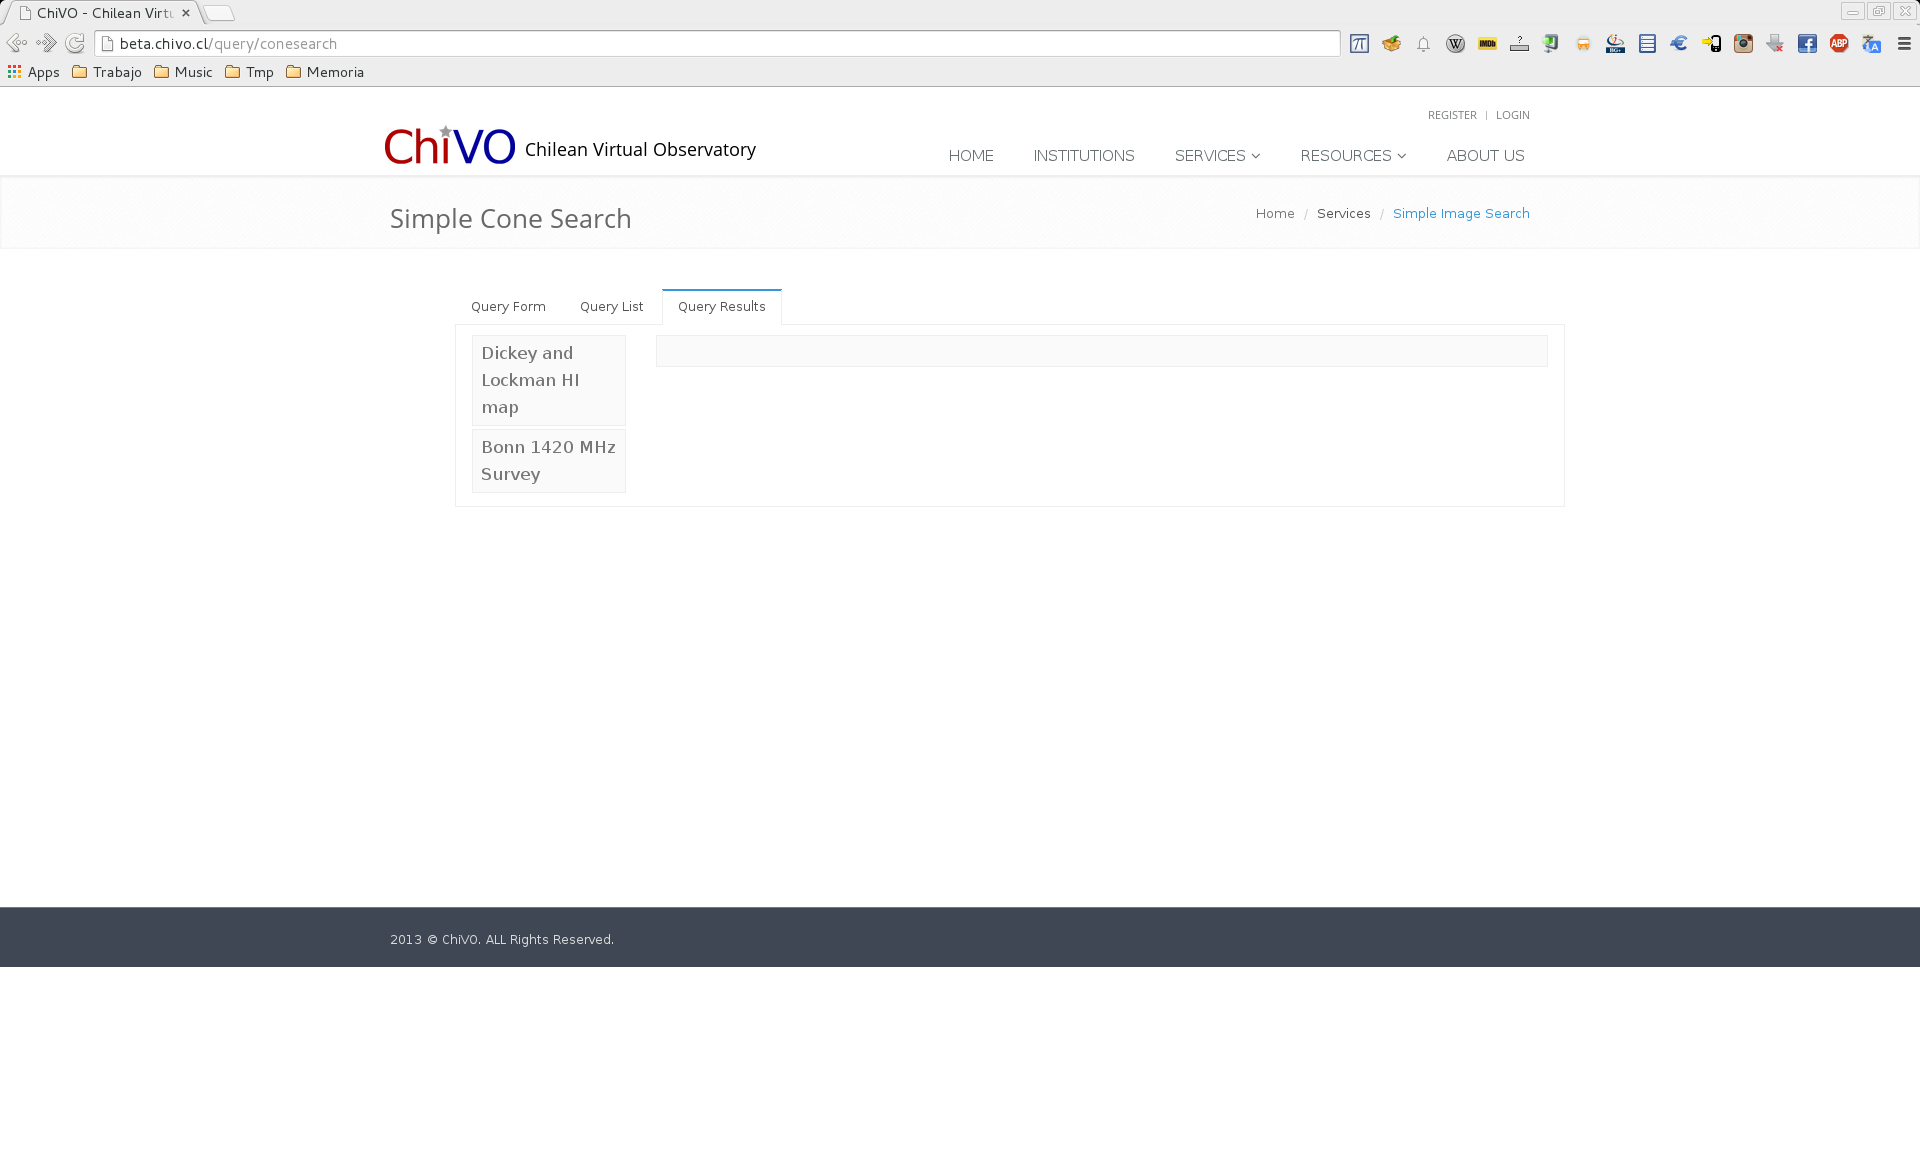
\includegraphics[scale=.2]{img/qrscs}
    \end{center}
    \caption{\emph{Query Results} para una búsqueda en SCS.}
    \label{img:qrscs}
\end{figure}

Finalmente, se debe presionar una de las dos fuentes para obtener los
resultados de la búsqueda. No obstante aquello, el listado de
resultados por fuentes siempre estará disponible en la barra lateral
izquierda, por lo que una vez seleccionada una fuente para ver los
resultados, se puede seleecionar otra para ver otros resultados.
Además, se puede seleccionar desde 1 hasta todas las fuentes
disponibles. En este caso, se ha seleccionado la fuente \emph{fuente},
la cual despliega un total de 4877 resultados, como se muestra en la
Fig.~\ref{img:qrscsvot}.

\begin{figure}[ht!]
    \begin{center}
	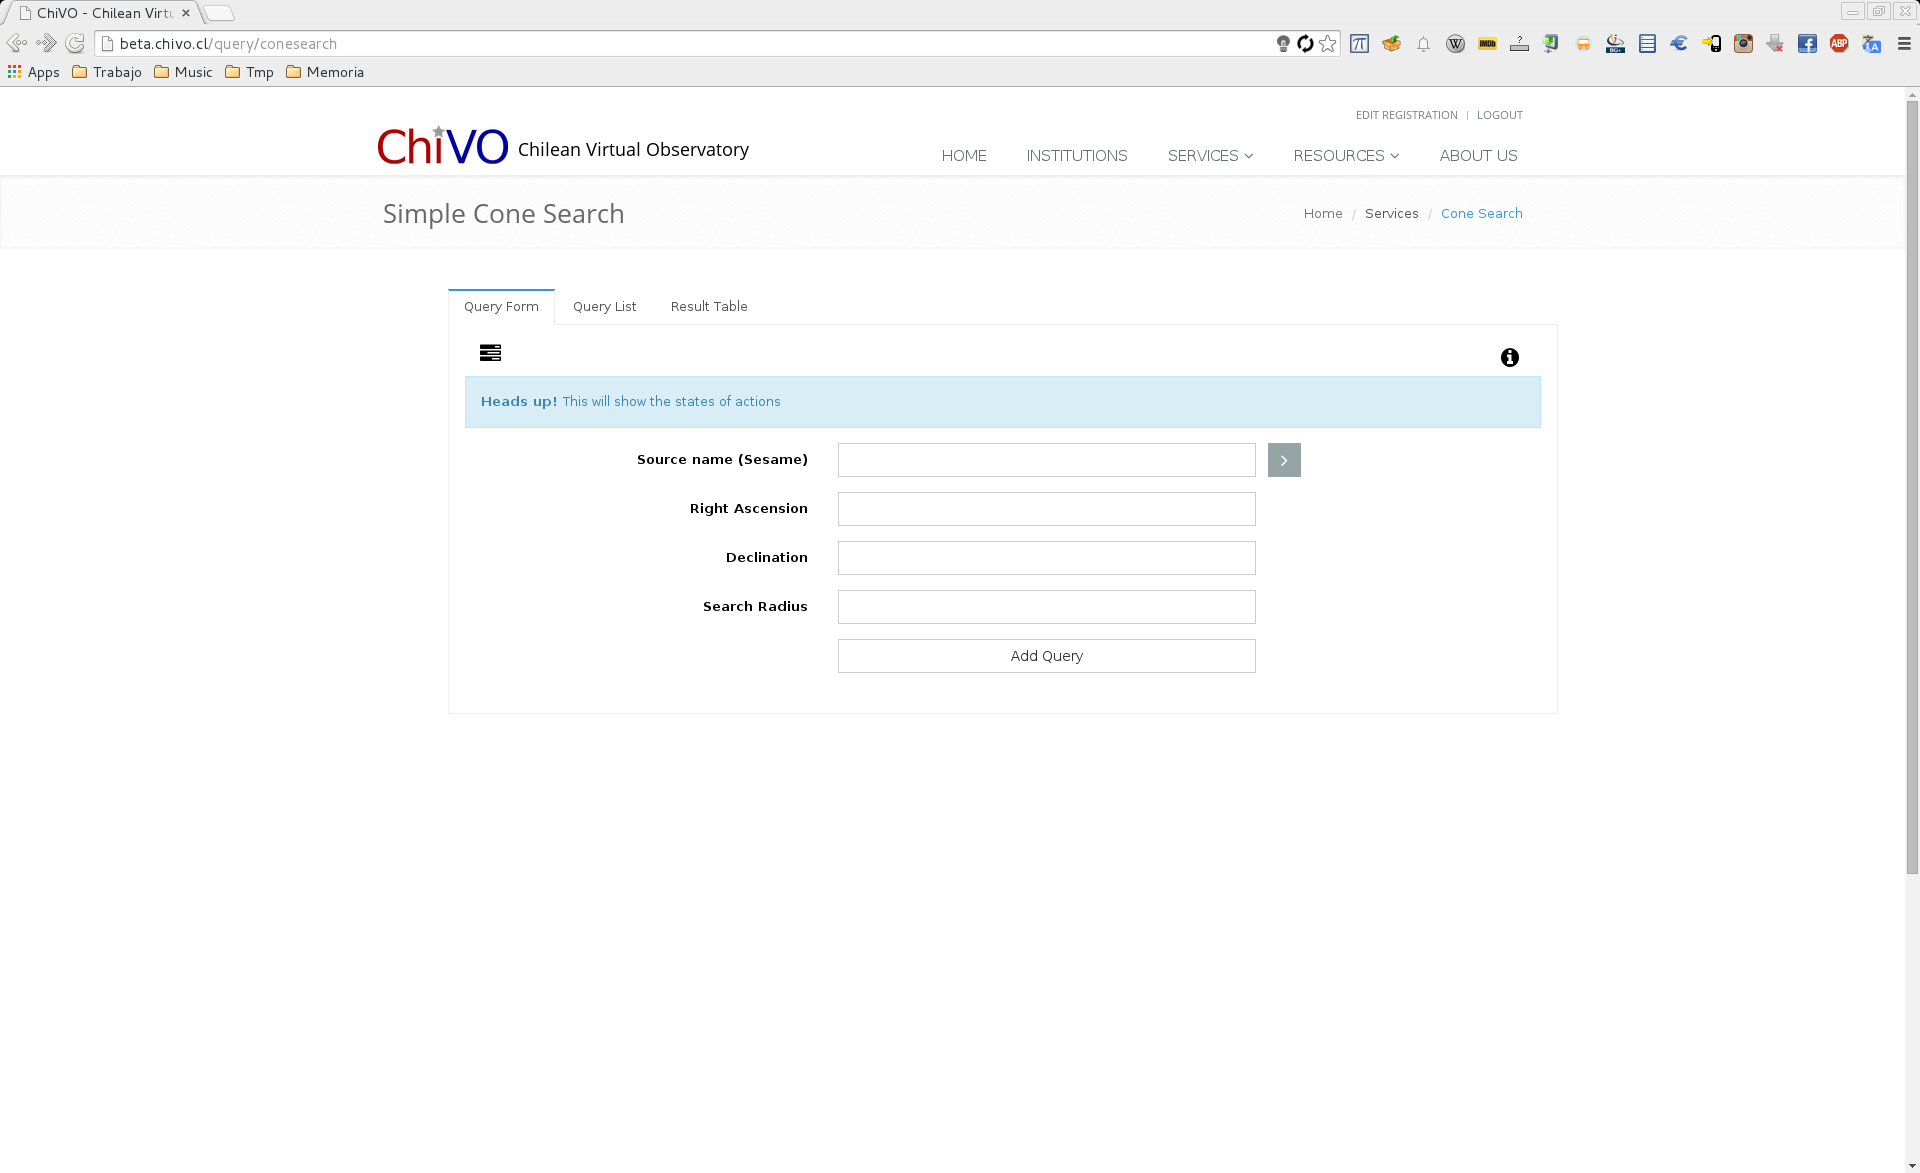
\includegraphics[scale=.2]{img/qrscsvot}
    \end{center}
    \caption{\emph{VO Table} para una búsqueda en SCS.}
    \label{img:qrscsvot}
\end{figure}



\paragraph{Simple Image Access}

Para este ejemplo se utilizará los siguientes datos:

\begin{description}
  \item [Source name (Sesame):] cygnus.
  \item [RA:] 299.86815263.
  \item [DEC:] 40.73391583
  \item [Angular Size:] 10.
\end{description}

Cabe recordar que al ingresar el campo Sesame, no es necesario
ingresar RA \& DEC, pues el sistema proveerá esos datos.

Al agregar esta consulta (presionando botón \emph{Add Query}), se puede
ir a la pestaña \emph{Query List} y revisar las fuentes disponibles.
Para este ejemplo se utilizará sólo dos fuentes para mostrar los
resultados. Para ello, de la lista de fuentes en la columna
\emph{Sources}, se seleccionará las siguientes:

\begin{itemize}
  \item PSPC summed pointed observations, 1 degree cutoff.
  \item Chandra Transmission Grating Catalog and Archive, Simple Image
    Access Interface.
\end{itemize}

Luego de seleccionar estas dos fuentes, se debe presionar el botón
\emph{process}, para luego pasar a la pestaña \emph{Query Results},
donde se encontrarán las dos fuentes seleccionadas, como lo muestra la
Fig.~\ref{img:qrsia}.

\begin{figure}[ht!]
    \begin{center}
	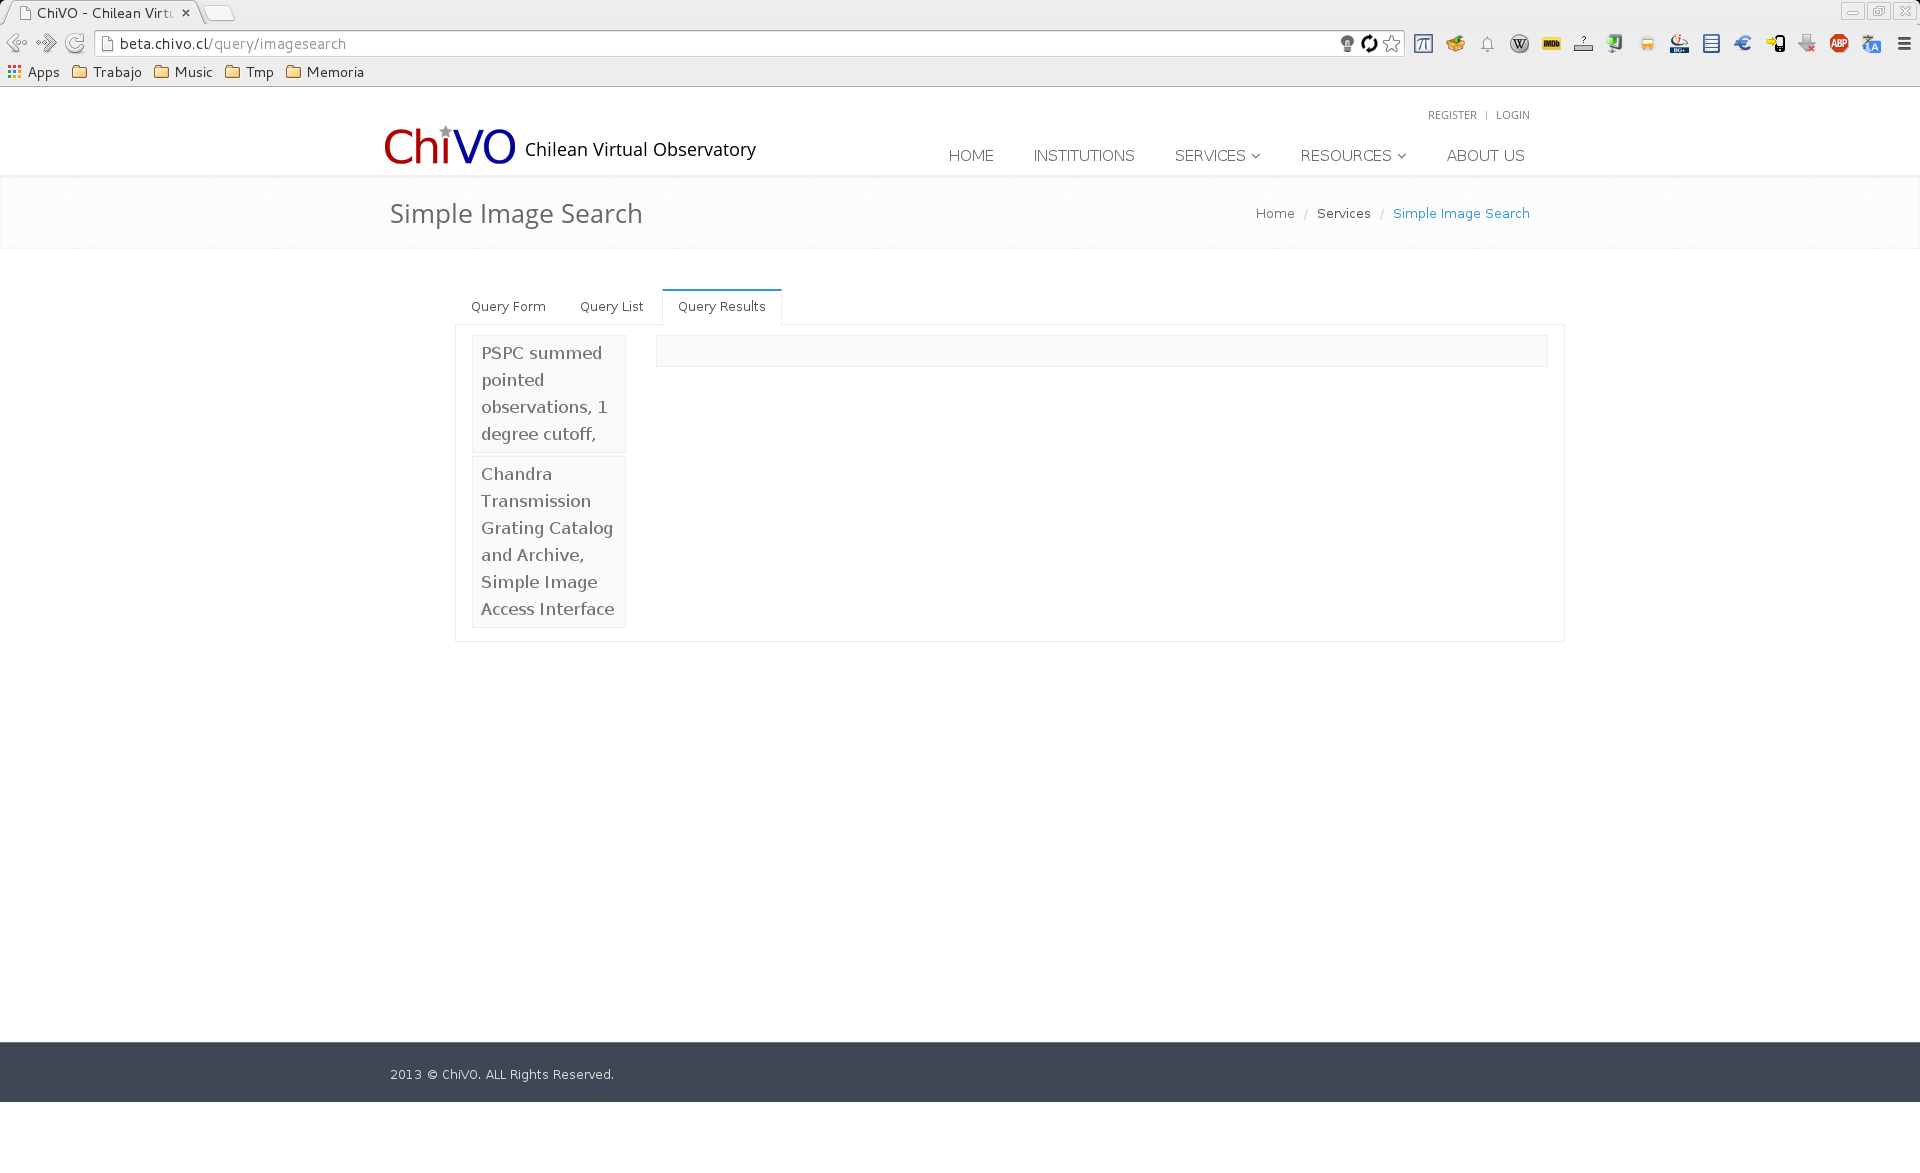
\includegraphics[scale=.2]{img/qrsia}
    \end{center}
    \caption{\emph{Query Results} para una búsqueda en SIA.}
    \label{img:qrsia}
\end{figure}

Finalmente, se debe presionar una de las dos fuentes para obtener los
resultados de la búsqueda. No obstante aquello, el listado de
resultados por fuentes siempre estará disponible en la barra lateral
izquierda, por lo que una vez seleccionada una fuente para ver los
resultados, se puede seleecionar otra para ver otros resultados.
Además, se puede seleccionar desde 1 hasta todas las fuentes
disponibles. En este caso, se ha seleccionado la fuente
\emph{Chandra Transmission Grating Catalog and Archive}, la cual
despliega un total de 147 resultados, como se muestra en la
Fig.~\ref{img:qrsiavot}.

\begin{figure}[ht!]
    \begin{center}
	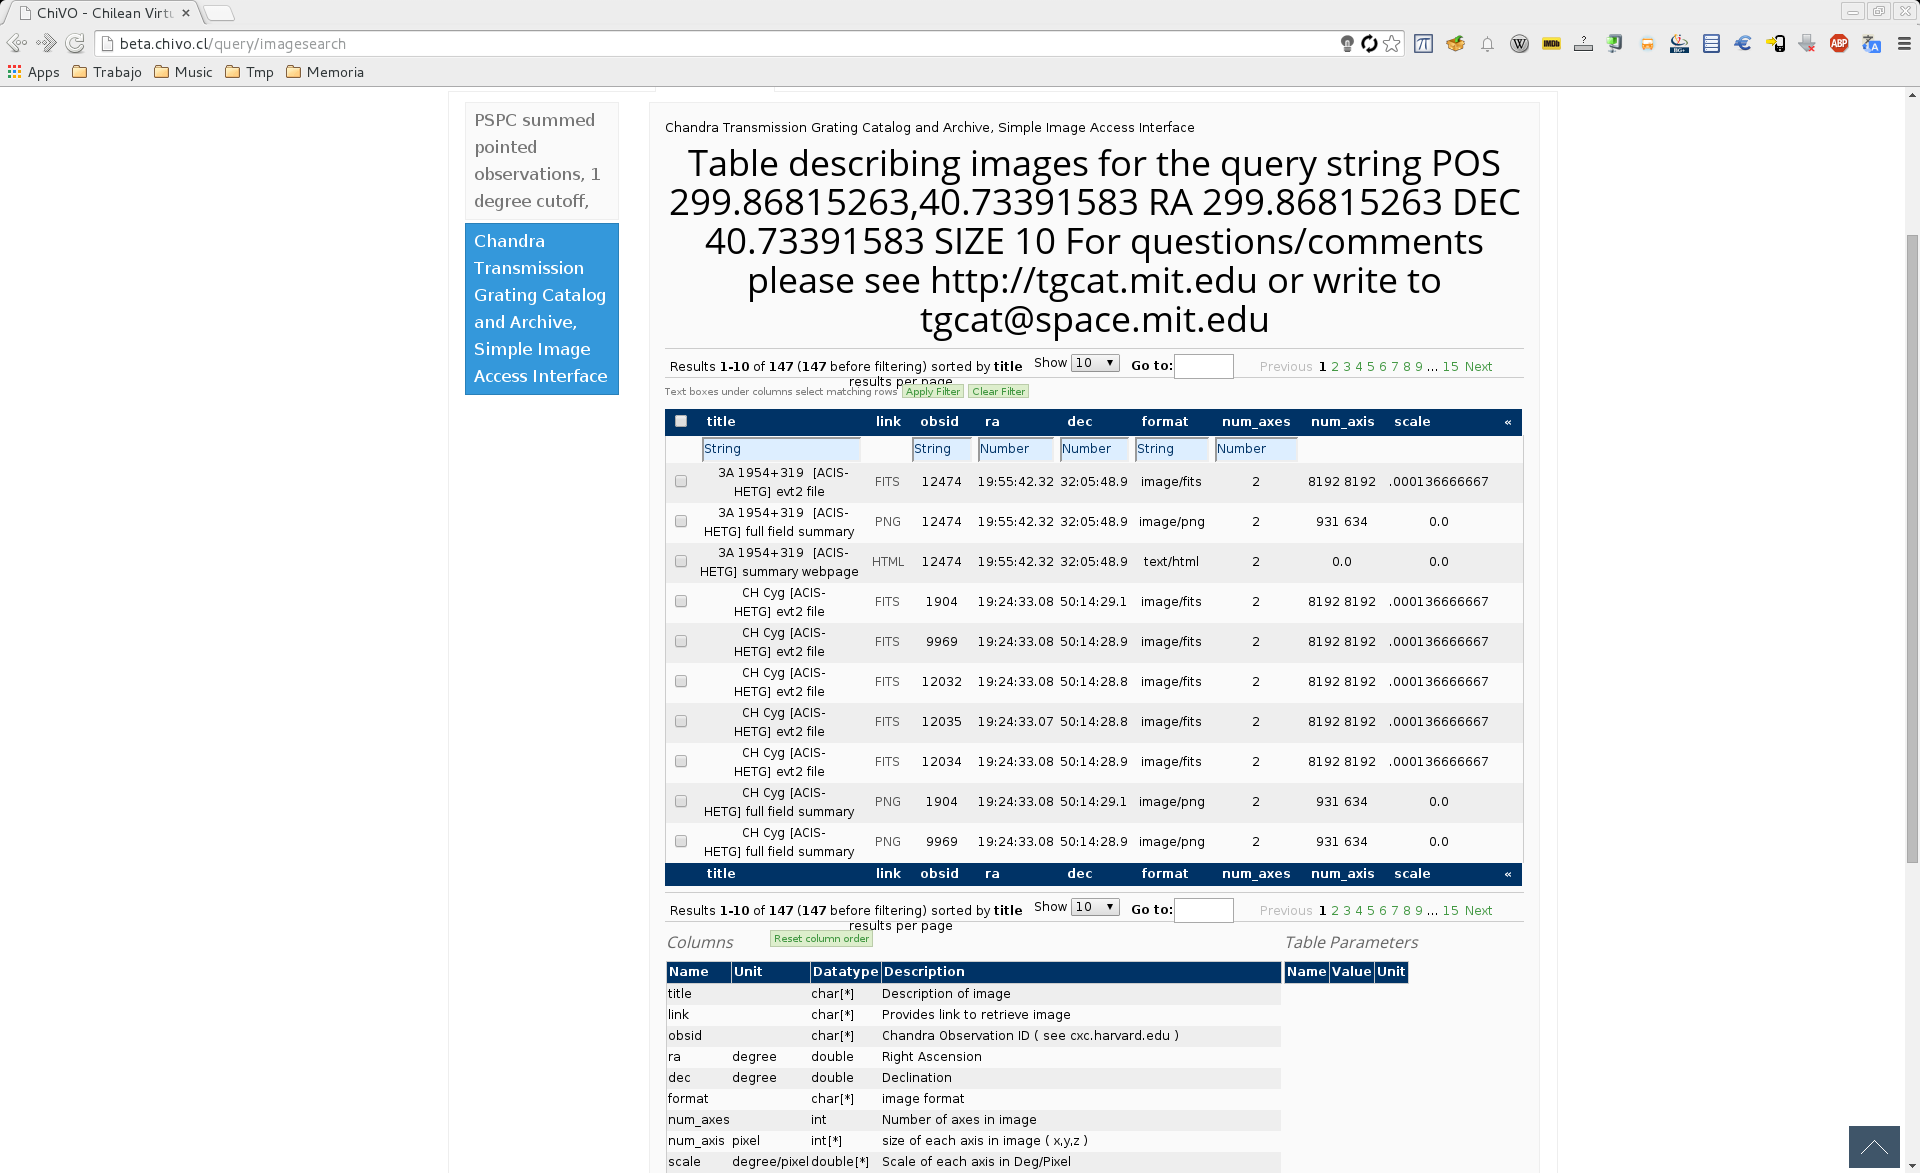
\includegraphics[scale=.2]{img/qrsiavot}
    \end{center}
    \caption{\emph{VO Table} para una búsqueda en SIA.}
    \label{img:qrsiavot}
\end{figure}


\paragraph{Simple Spectral Access}

Para este ejemplo se utilizará los siguientes datos:

\begin{description}
  \item [Source name (Sesame):] orion.
  \item [RA:] 83.82208333.
  \item [DEC:] -5.39111111.
  \item [Size:] 50.
\end{description}

Cabe recordar que al ingresar el campo Sesame, no es necesario
ingresar RA \& DEC, pues el sistema proveerá esos datos. Los campos
\emph{band} y \emph{time} son opcionales y sirven para refinar la
búsqueda. Para este caso no se utilizarán (se dejan en blanco) para
obtener mayores resultados.

Al agregar esta consulta (presionando botón \emph{Add Query}), se puede
ir a la pestaña \emph{Query List} y revisar las fuentes disponibles.
Para este ejemplo se utilizará sólo dos fuentes para mostrar los
resultados. Para ello, de la lista de fuentes en la columna
\emph{Sources}, se seleccionará las siguientes:

\begin{itemize}
  \item Wisconsin Ultraviolet Photo-Polarimeter Experiment.
  \item ELODIE archive.
\end{itemize}

Luego de seleccionar estas dos fuentes, se debe presionar el botón
\emph{process}, para luego pasar a la pestaña \emph{Query Results},
donde se encontrarán las dos fuentes seleccionadas, como lo muestra la
Fig.~\ref{img:qrssa}.

\begin{figure}[ht!]
    \begin{center}
	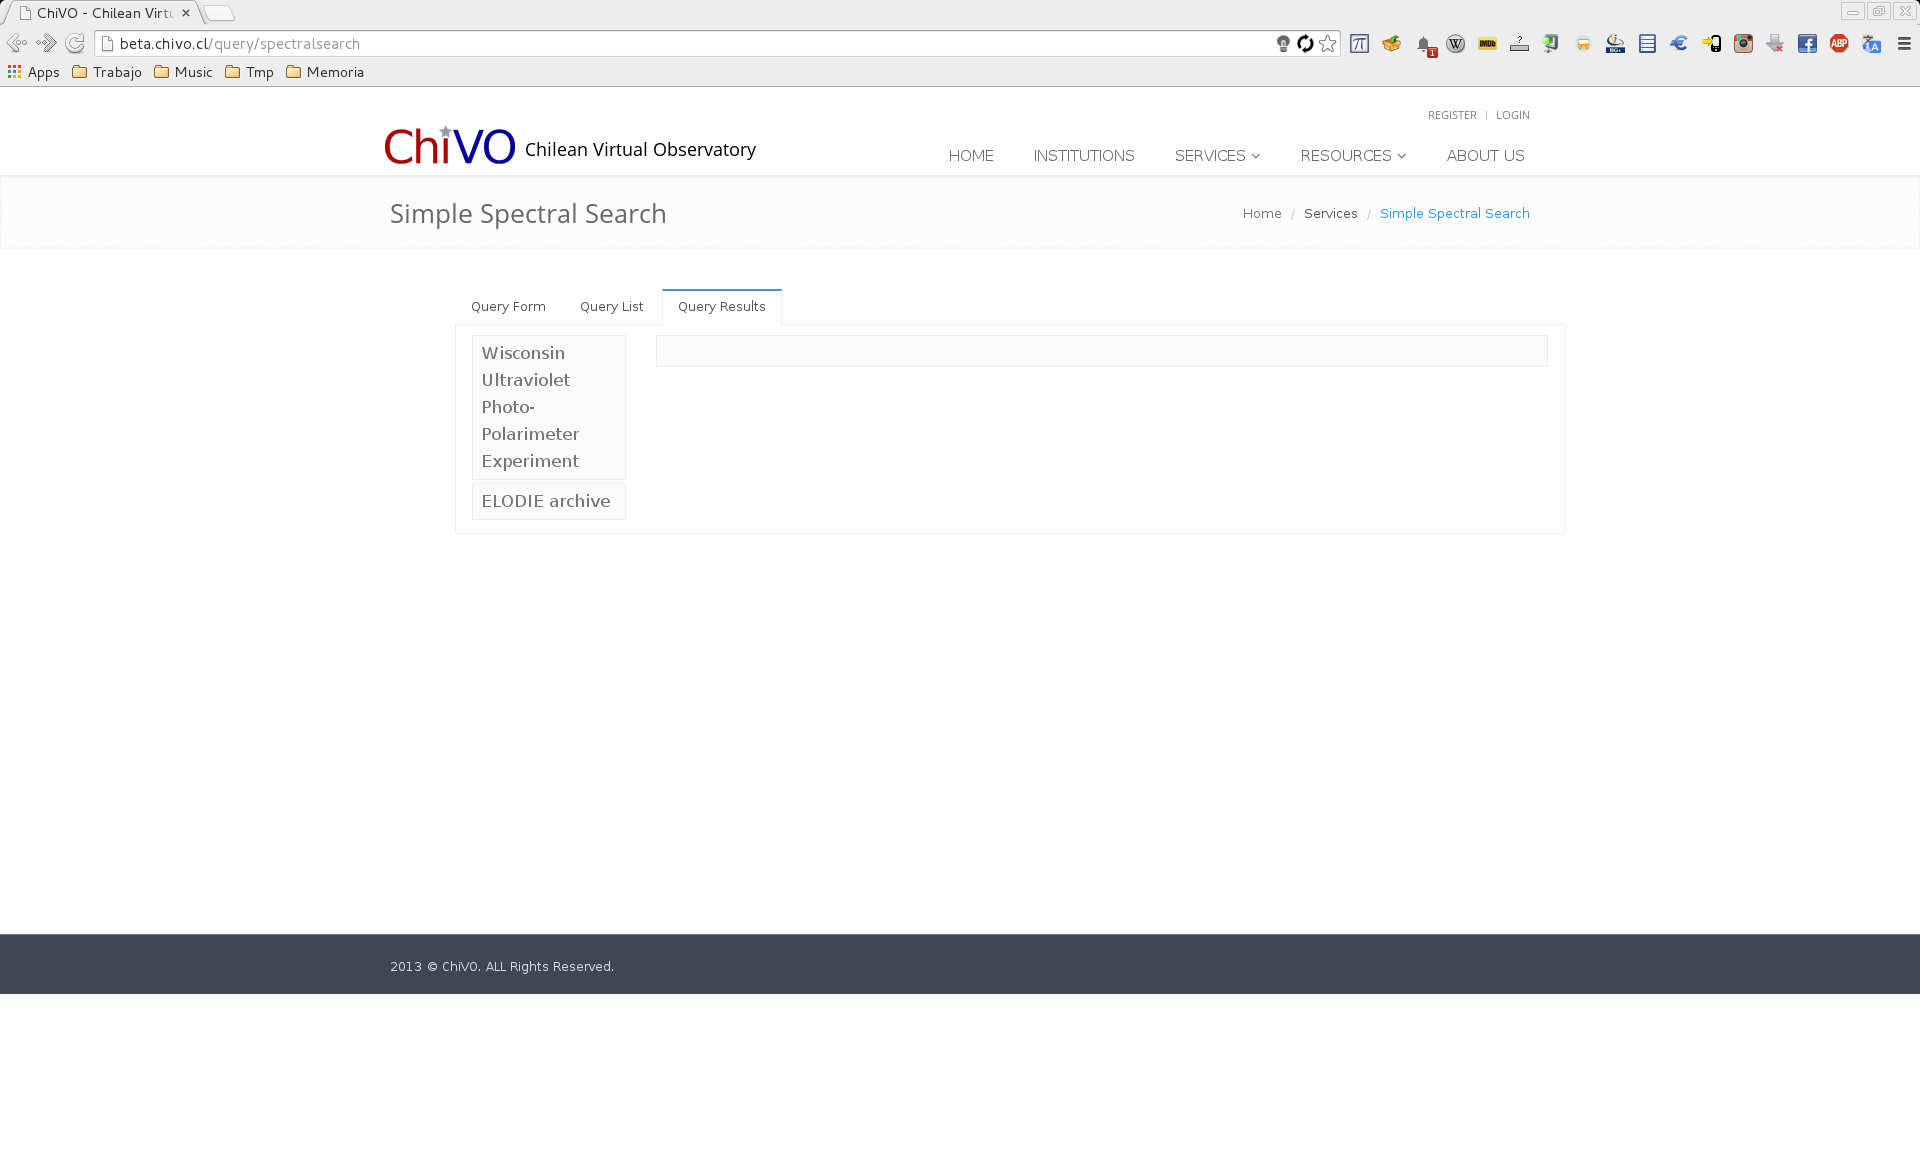
\includegraphics[scale=.2]{img/qrssa}
    \end{center}
    \caption{\emph{Query Results} para una búsqueda en SSA.}
    \label{img:qrssa}
\end{figure}

Finalmente, se debe presionar una de las dos fuentes para obtener los
resultados de la búsqueda. No obstante aquello, el listado de
resultados por fuentes siempre estará disponible en la barra lateral
izquierda, por lo que una vez seleccionada una fuente para ver los
resultados, se puede seleecionar otra para ver otros resultados.
Además, se puede seleccionar desde 1 hasta todas las fuentes
disponibles. En este caso, se ha seleccionado la fuente \emph{ELODIE
archive}, la cual despliega un total de 4877 resultados, como se
muestra en la Fig.~\ref{img:qrssavot}.

\begin{figure}[ht!]
    \begin{center}
	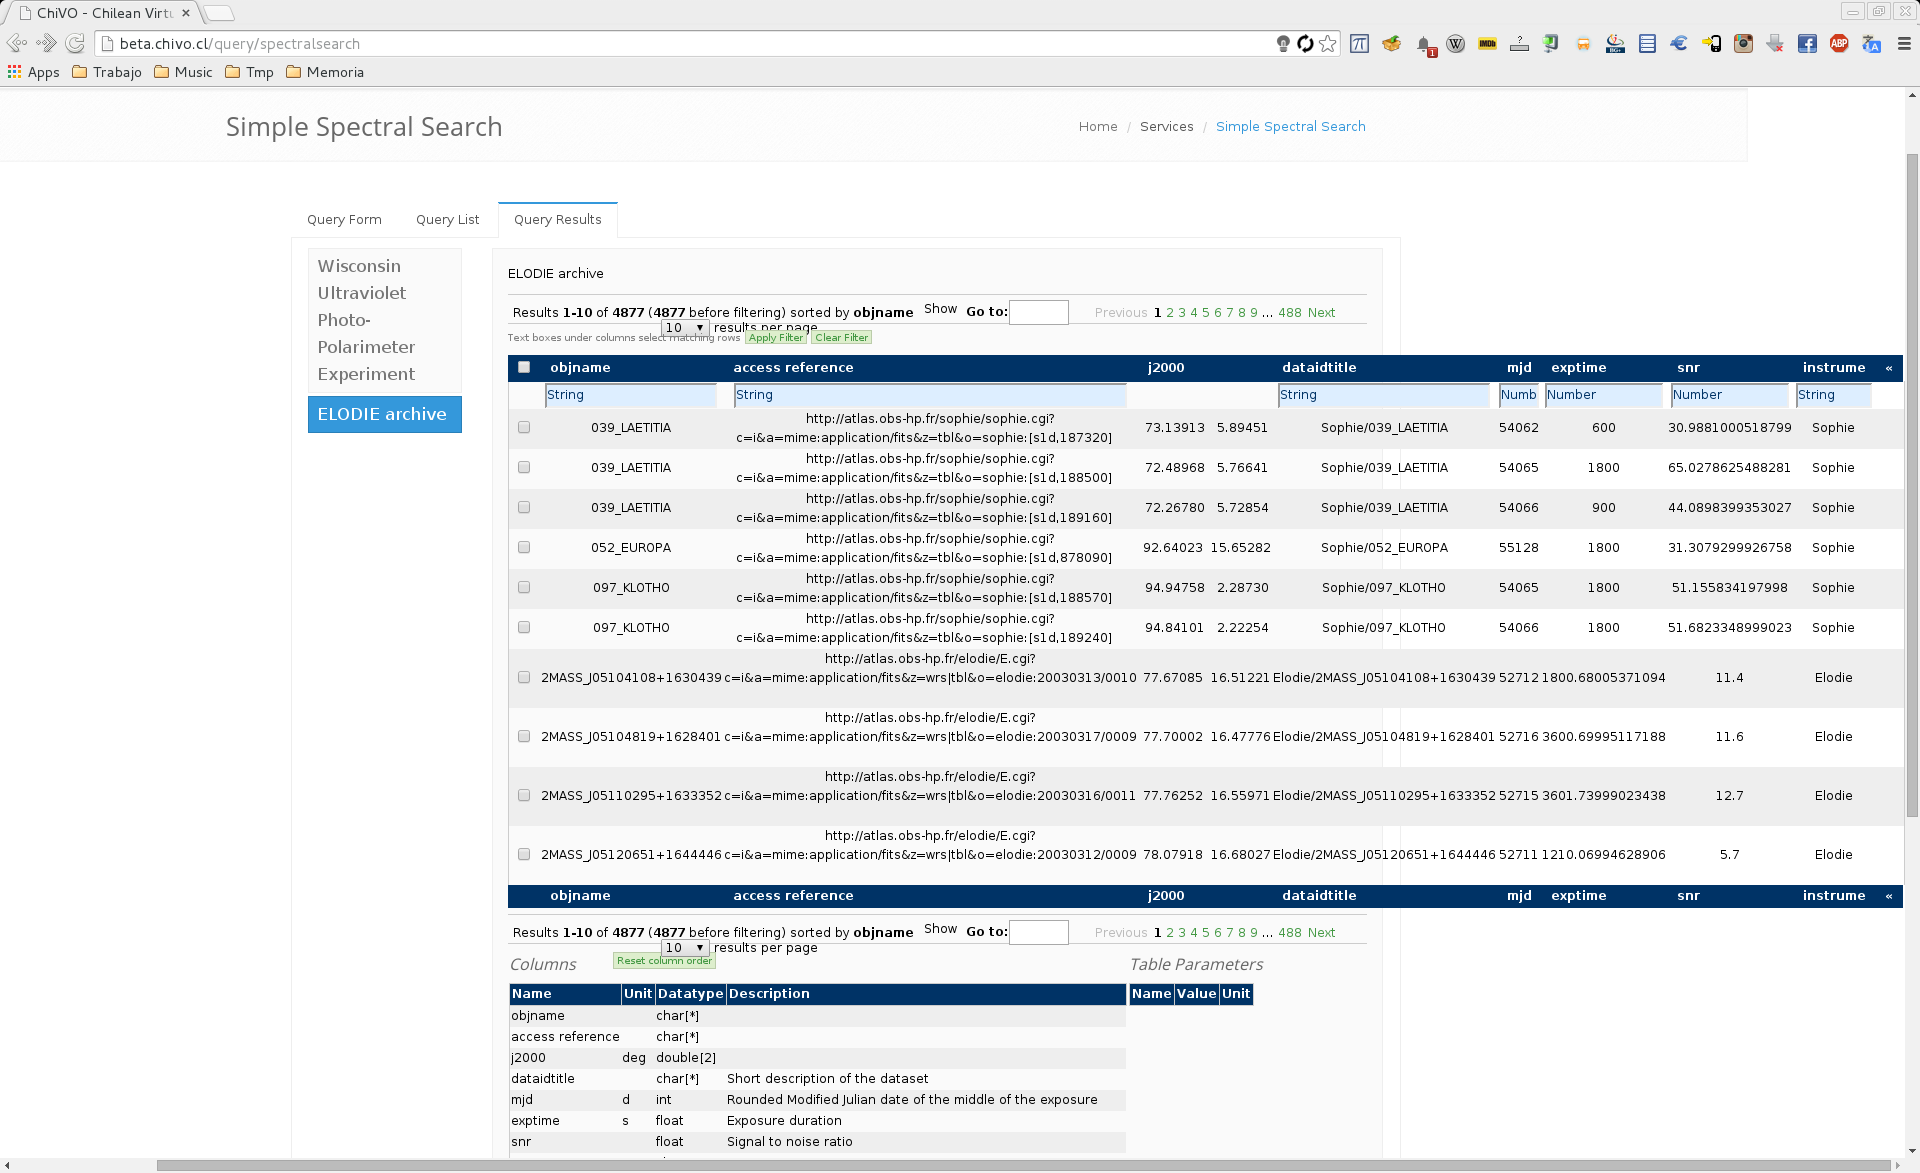
\includegraphics[scale=.2]{img/qrssavot}
    \end{center}
    \caption{\emph{VO Table} para una búsqueda en SSA.}
    \label{img:qrssavot}
\end{figure}

